%\pdfminorversion=4
\documentclass[xcolor=svgnames,12pt]{beamer}

\let\Tiny=\tiny % fuck you dolphin !

\usepackage[utf8]{inputenc}
\usepackage[french]{babel}
\usepackage{lmodern}
\usepackage[T1]{fontenc}
\usepackage{graphicx} % pix

%
% THEME
%
\usetheme{Bergen}
\def\insertauthorindicator{Qui}
\def\insertinstituteindicator{Où}
\def\insertdateindicator{Quand}% Default is "When?"
\useinnertheme{rectangles}
\usecolortheme{orchid}
\setbeamertemplate{navigation symbols}{} % pas de symboles merdiques en bas
\fontsize{6pt}{7.2}\selectfont

%
% META
%
\title{Git en projet: le kit de survie.}
\subtitle{Comment éviter les coups de bâtons}
\author{Julien (jvoisin) Voisin}
\date{\today{}}
\institute{hackgyver (Belfort)}

%
% DOCUMENT
%
\begin{document}
\begin{frame}
    \maketitle
\end{frame}

\begin{frame}
    \tableofcontents
\end{frame}

\begin{frame}{Experiences}
    \begin{block}{Bonheur}
    \begin{itemize}[<+->]
            \item Gestion des fusions
            \item Nomade
            \item Traçabilité
            \item Non-répudiation
        \end{itemize}
    \end{block}
\end{frame}

\begin{frame}{Disclamer}
    \begin{itemize}
        \item Les images de ce diapo ont été honteusement piquées sur git-pro.
        \item Je n'ai jamais utilisé subversion.
    \end{itemize}
\end{frame}

\section{Qu'est-ce que c'est ?}
\subsection{Un truc super.}
\begin{frame}{Git, cet inconnu}
    \begin{block}{Historique}
        \begin{itemize}
            \item Pour commencer étaient les mails (1991--2002),
            \item puis vint Bitkeeper (2002--2005),
            \item et enfin, git fût.
        \end{itemize}
    \end{block}
    \pause
    \begin{block}{Conception}
        \begin{itemize}
            \item Distribué
            \item Rapide
            \item Incorruptible
        \end{itemize}
    \end{block}
\end{frame}

\section{À quoi ça sert ?}
\subsection{Éviter les coups de bâtons.}

\begin{frame}{Mais moi j'utilise}
    \begin{itemize}
        \item Dropbox
        \item Des mails
        \item Un ftp
        \item Une clef USB
    \end{itemize}
    \pause
    \hspace{1cm}
    \begin{center}
        \huge Coups de bâton.
    \end{center}
\end{frame}

\begin{frame}{Pourquoi git est mieux}
    \begin{block}{Parce qu'il}
        \begin{itemize}
            \item est libre.
            \item gère l'historique des versions.
            \item gère les branches.
            \item gère les conflits.
            \item est scalable.
            \item est intègre.
        \end{itemize}
    \end{block}
\end{frame}

\begin{frame}{Fonctionnement interne}
    \begin{block}{Technique}
        \begin{itemize}
            \item Snapshots vs. diff
            \item "Pointeurs"
            \item Tout (ou presque) peut se faire en local
        \end{itemize}
    \end{block}
\end{frame}


\section{Comment ça s'utilise ?}
\subsection{Bien.}
\begin{frame}{La vie des fichiers}
    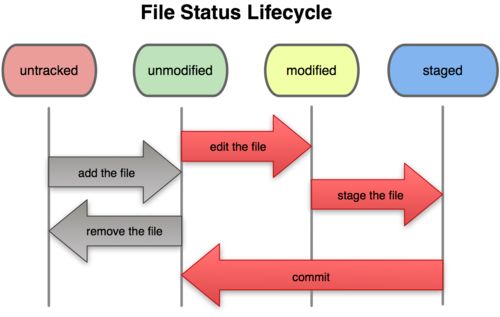
\includegraphics[width=.7\paperwidth]{file.png}
\end{frame}

\begin{frame}{Gérer les fichiers}
    \begin{block}{Modifier}
        \begin{itemize}
            \item git diff
            \item git status
            \item git add/rm/mv
            \item git commit
        \end{itemize}
    \end{block}
\end{frame}

\begin{frame}{Les branches}
    \begin{block}{Créer}
        \begin{itemize}
            \item git branch
            \item git branch -d
            \item git checkout
        \end{itemize}
    \end{block}
    \pause
    \begin{block}{Fusionner}
        \begin{itemize}
            \item git merge
            \item git merge-tool
            \item git cherry-pick
        \end{itemize}
    \end{block}
\end{frame}

\begin{frame}{L'enfer, c'est les autres}
    \begin{block}{Partager}
        \begin{itemize}
            \item git clone url
            \item git fetch
            \item git pull
            \item git push
            \item git remote add/remove name url
        \end{itemize}
    \end{block}
    \pause
    \begin{block}{Bâtonner}
        \begin{itemize}
            \item git revert
            \item git log
            \item git blame
        \end{itemize}
    \end{block}
\end{frame}

\begin{frame}{Workflow}
    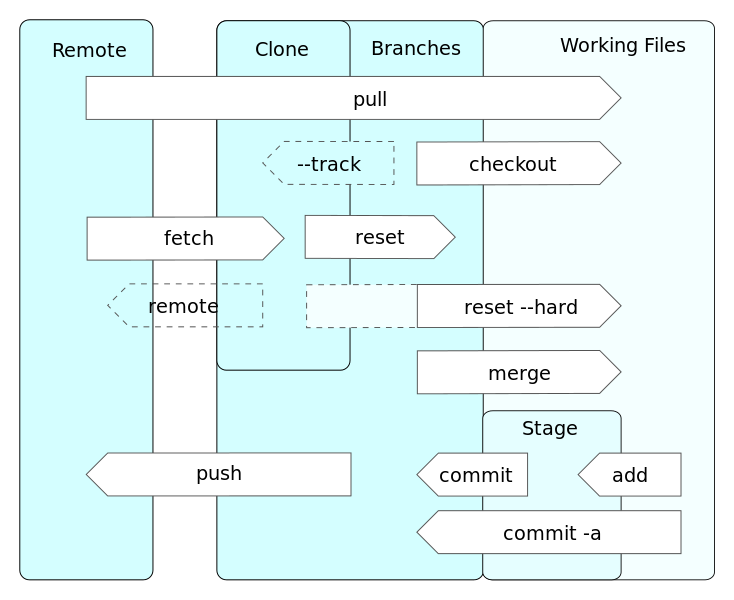
\includegraphics[width=.7\paperwidth]{flow.png}
\end{frame}

\begin{frame}{Baluchon}
    \begin{block}{A connaitre}
    \begin{itemize}
        \item Pro git
        \item Gitg et meld
        \item man git-*
    \end{itemize}
    \end{block}
\end{frame}

\begin{frame}{Question ?}
    
\includegraphics[width=.7\paperwidth]{baton.jpg}
\end{frame}

\end{document}
